\section{Modification of the \qs{} long edge representation}
\label{qsr}
\subsection{\qsr{}}

An implementation of \qs{} with a modified approach to representing insignificant bits for a node in the \qt{} has been implemented in \texttt{qsr.cpp} and is called \qsr{}. Section \ref{finding_improvements} described the method for getting to this, and this section will properly introduce the extension to the algorithm and why it should yield practical improvements in some scenarios.
\\
\\
This experiment focuses on the pruning step of the algorithm. Recall that in the pruning step \qs{} shifts each point in a quad towards the lower left corner by replacing existing bits with zero's. The alteration introduced in this experiment moves each point in a quad towards a random corner of that quad. More precisely, by not only introducing zero's into the bit string as replacement, this feature insert bits into the bit string at random. The modification in the implementation is subtle and is illustrated in listing \ref{lst:qsr} below, which is extracted from lines 91-99 in \texttt{qsr.cpp}:

\begin{lstlisting}[caption={Pruning with random bits},label={lst:qsr}]
if (long_edge_length >= lambda && parts.size() == 1)
{
	if (rand()%2)
{
	new_p[j] += 1.0 / (2.0 * (1 << depth));
}
	continue;
}
new_p[j] += 1.0 / (2.0 * (1 << depth));
\end{lstlisting}

This will for each dimension of a node that is pruned, insert a bit at random, or else continue as in the original implementation. This might improve the resulting sketch by "pulling" the point in an arbitrary direction for each dimension rather than only distorting them in one direction. This could potentially improve some scenarios of the sketch where the points are either. A visualization of this can be seen on figure \ref{fig:randombits}, where the transformation by \qs{} is referred to as QS, and the transformation by \qsr{} is referred to as QSR. In the graphical representation each point lies next to each other if they are placed in the same corner, where in the actual transformation these will have the exact same coordinates. 
\begin{figure}[h]
	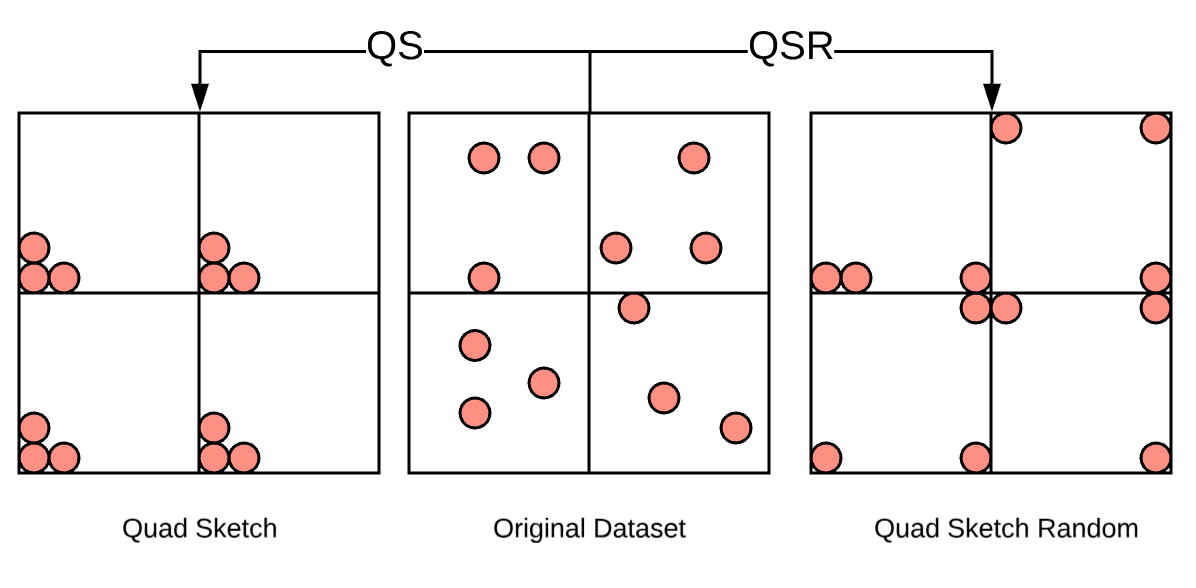
\includegraphics[width=1\textwidth]{figures/randombits}
	\caption{Random Bit Demonstration}
	\label{fig:randombits}
\end{figure}
The given example in figure \ref{fig:randombits} demonstrates a scenario where the experiment performs decently. It should be noted that the random movement of the points could also result in a worse representation. Such a scenario is discussed in \ref{disc/threats/randomness}.
\\
\\
The motivation of this experiment stems from the creation of the random quad tree in \qs{}. Should the creation of this \qt{} accidentally quad through closely clustered points then the distortion could be quite severe. By introducing randomness into the direction of the points, they might end up in corners closer to each other and thereby reduce the amount of distortion.

\subsection{Expected value}
Consider some bitstring \textit{B} of length \textit{n} which has been removed by \qs{} pruning for one dimension. Let \textit{k} = $2^n$ describe the range of \textit{B}. The expected average euclidean distance \textit{$d_B$} from the bitstring of zero's inserted by \qs{} to \textit{B} can be formalized as\footnote{\url{https://en.wikipedia.org/wiki/Expected_value\#Finite_case}}:
\\
$$E[\textit{$d_B$}] = \sum_{i=0}^{k - 1} \dfrac{i}{k}$$
\\
%\textit{$d_B$} can as such be reduced to $\dfrac{k-1}{2}$
The expected average euclidean distance \textit{$d'_B$} from B to the bitstring inserted by \qsr{} can be described as the distance from B to some random bitstring \textit{B'} with the same length \textit{n}. There are k different values for \textit{B} and for each of these some distance to the k different values for \textit{B'}. This gives ac collection of distances \textit{D} of length $k^2$ where $\forall{}\textit{d}\in{}\textit{D}$ $0\leq{}d\leq{}k-1$. As such \textit{$d'_B$} can be formalized as:
\\
$$E[\textit{$d'_B$}] = \sum_{d\in\textit{D}}^{}\dfrac{d}{k^2}$$
\\
